\chapterp{3p}{Online band-pass filters}\label{ch:BPF}

This section explores the current state-of-the-art method in online SWR detection. This method is very similar to the procedure for offline ripple detection described in \cref{ch:offline}: we also select a single recording channel containing ripples, band-pass filter its data through the ripple band, and apply a detection threshold to the envelope of the filter output.

The difference is that the SWR detection must now happen under real-time constraints. No future samples $\z_{t_f}$ can be used when deciding whether the recording sample $\z_t$ ($t < t_f$) belongs to an SWR event.

In other words, the band-pass filter has to be causal. It also means that we can no longer use the Hilbert transform to calculate the envelope $n_t$ of the band-pass filter output $o_t$. In practice, the band-pass filter output is often simply rectified (i.e. $n_t = \abs{o_t}$). Although the resulting jagged signal is not as visually pleasing as the Hilbert-transform based envelope, it is effective for signal detection. (\Citeauthor{Sethi2014} showed that more advanced online envelope estimators did not yield better detection performance \cite{Sethi2014}).

% \Cref{ch:eval} showed how we form detections 

% continue: what's used in online SWR-detection literature.

% continue: for each filter, a separate plot (in appendix) of its parameter range (rp, rs, width). DONE
% continue: a plot of groupdelay in ripple band, and ratio of sumated magnitude responses passband versus stopband. DONE
% continue: lit filters.
%   Dutta: 30-tap FIR
%   


\clearpage
\begin{figure}
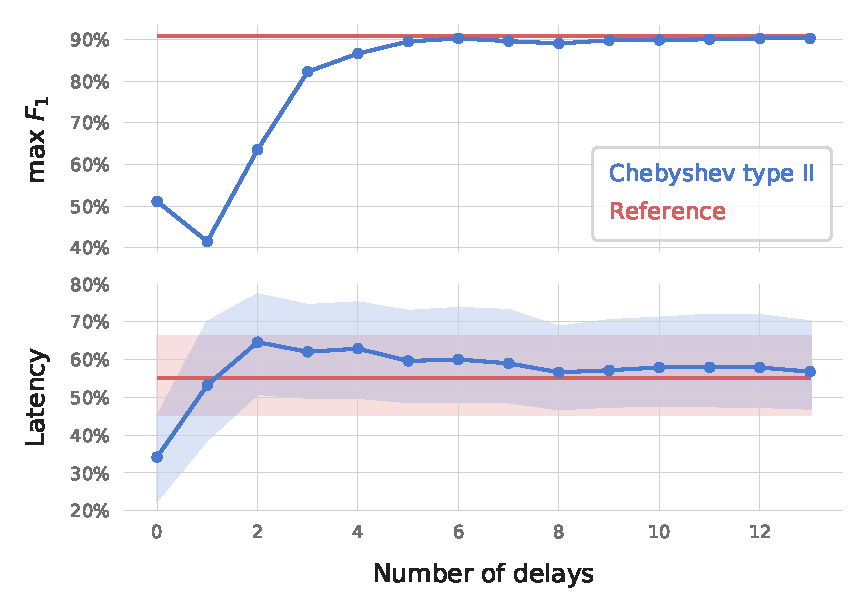
\includegraphics{figures/searcharray-cheby2}
\captionn[, ]{Performance of Chebyshev type 2 IIR-filters}{for different filter orders. The minimum stop-band attenuation was set to 40 dB.}
\end{figure}

\begin{figure}
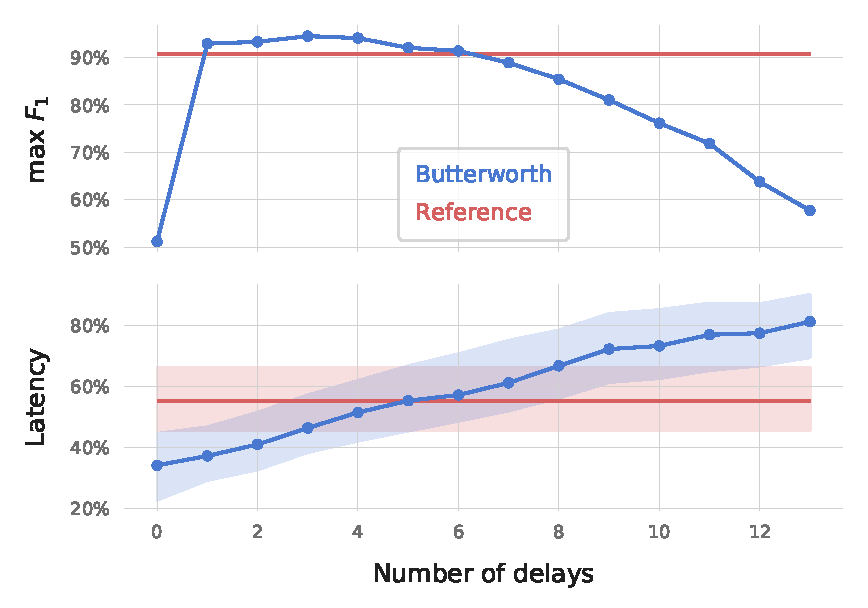
\includegraphics{figures/searcharray-butter}
\captionn[, ]{Performance of Butterworth IIR-filters}{for different filter orders.}
\end{figure}
